%% This is a tikz file

% This file is set up to use 11pt palatino font.
\tikzset{node lower left/.style={font=\scriptsize,anchor=north east,yshift=-0.032cm,text height=0.198cm,text depth=0.079cm,inner sep=0.03cm},
leaf/.style={font=\normalsize,anchor=west,text height=0.271cm,text depth=0.109cm,inner sep=0.13cm},
node upper left/.style={font=\scriptsize,anchor=south east,yshift=-0.032cm,text height=0.198cm,text depth=0.079cm,inner sep=0.03cm},
bracket label/.style={font=\normalsize,anchor=west,text height=0.271cm,text depth=0.109cm,inner sep=0.2cm},
node upper right/.style={font=\scriptsize,anchor=south west,text height=0.198cm,text depth=0.079cm,inner sep=0.03cm},
node right/.style={font=\scriptsize,anchor=west,text height=0.198cm,text depth=0.079cm,inner sep=0.03cm},
branch/.style={font=\tiny,text height=0.149cm,text depth=0.059cm,inner sep=0.025cm},
root/.style={font=\normalsize,anchor=east,text height=0.271cm,text depth=0.109cm},
node lower right/.style={font=\scriptsize,anchor=north west,text height=0.198cm,text depth=0.079cm,inner sep=0.03cm}}
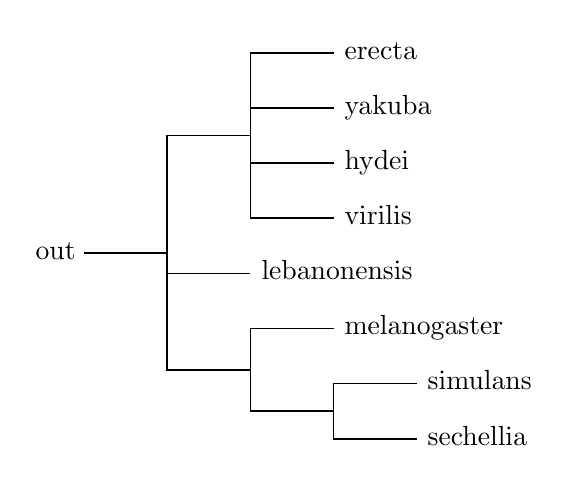
\begin{tikzpicture}[semithick,inner sep=0.1cm]
%                         +---------7:erecta
%                         |
%                         |---------8:yakuba
%               +---------6
%               |         |---------9:hydei
%               |         |
%               |         +---------10:virilis
% out:11--------5
%               |---------12:lebanonensis
%               |
%               |         +---------4:melanogaster
%               +---------3
%                         |         +----------1:simulans
%                         +---------0
%                                   +----------2:sechellia

% The scale is 10.552500, and the yScale is 0.700000

%% Coordinates of nodes.
\coordinate (n11) at (0.000,2.362);
\coordinate (n5) at (1.055,2.362);
\coordinate (n5p) at (0.000,2.362);
\coordinate (n6) at (2.111,3.850);
\coordinate (n6p) at (1.055,3.850);
\coordinate (n7) at (3.166,4.900);
\coordinate (n7p) at (2.111,4.900);
\coordinate (n8) at (3.166,4.200);
\coordinate (n8p) at (2.111,4.200);
\coordinate (n9) at (3.166,3.500);
\coordinate (n9p) at (2.111,3.500);
\coordinate (n10) at (3.166,2.800);
\coordinate (n10p) at (2.111,2.800);
\coordinate (n12) at (2.111,2.100);
\coordinate (n12p) at (1.055,2.100);
\coordinate (n3) at (2.111,0.875);
\coordinate (n3p) at (1.055,0.875);
\coordinate (n4) at (3.166,1.400);
\coordinate (n4p) at (2.111,1.400);
\coordinate (n0) at (3.166,0.350);
\coordinate (n0p) at (2.111,0.350);
\coordinate (n1) at (4.221,0.700);
\coordinate (n1p) at (3.166,0.700);
\coordinate (n2) at (4.221,0.000);
\coordinate (n2p) at (3.166,0.000);

%% horizontal lines
\draw (n5p) -- (n5);
\draw (n6p) -- (n6);
\draw (n7p) -- (n7);
\draw (n8p) -- (n8);
\draw (n9p) -- (n9);
\draw (n10p) -- (n10);
\draw (n12p) -- (n12);
\draw (n3p) -- (n3);
\draw (n4p) -- (n4);
\draw (n0p) -- (n0);
\draw (n1p) -- (n1);
\draw (n2p) -- (n2);

%% vertical lines
\draw [line cap=rect] (n6p) -- (n3p);
\draw [line cap=rect] (n7p) -- (n10p);
\draw [line cap=rect] (n4p) -- (n0p);
\draw [line cap=rect] (n1p) -- (n2p);

%% leaf labels
\node [leaf,text height=0.271cm,text depth=0.109cm] at (n7) {erecta};
\node [leaf,text height=0.271cm,text depth=0.109cm] at (n8) {yakuba};
\node [leaf,text height=0.271cm,text depth=0.109cm] at (n9) {hydei};
\node [leaf,text height=0.271cm,text depth=0.109cm] at (n10) {virilis};
\node [leaf,text height=0.271cm,text depth=0.109cm] at (n12) {lebanonensis};
\node [leaf,text height=0.271cm,text depth=0.109cm] at (n4) {melanogaster};
\node [leaf,text height=0.271cm,text depth=0.109cm] at (n1) {simulans};
\node [leaf,text height=0.271cm,text depth=0.109cm] at (n2) {sechellia};

%% root label
\node [root,text height=0.271cm,text depth=0.109cm] at (n11) {out};

\end{tikzpicture}
